\label{chap:cones}One of the most essential ingredients for the conception of the idea of holography was the fact that a stack of coincident D3-branes naturally features a 4D gauge theory on their world-volume, where the 4D fields emerge from the modes of open strings stretching between them. In the simplest and most famous example, a stack of $N$ D3-branes is placed in otherwise Minkowski $\mathbb{R}^{1,9}$; the corresponding field theory is the maximally supersymmetric Yang-Mills in four dimensions (\SYM).

Setting the stack on a different background geometry instead gives rise to a large family of different field theories; a particularly interesting subset is given by spacetimes of the form

\begin{equation} 
	M = \mathbb{R}^{1,3} \times X_6 \,,
\end{equation}

where the $\mathbb{R}^{1,3}$ is parallel to the branes (and must be identified with the field theory spacetime) and $X_6$ is a 6-dimensional Calabi-Yau cone over a compact 5-fold base $Y_5$. By $X_6$ being a cone it is meant there exists a conical radial coordinate $r$ such that the metric on $X_6$ is of the form

\begin{equation}
	ds^2 = dr^2 + r^2 ds_5^2
	\label{}
\end{equation}

With $ds_5^2$ the metric on $Y_5$.

In this language, the \SYM example above corresponds to $X_6 = \mathbb{R}^6 = \mathbb{C}^3$, which is (trivially) a cone over $Y_5 = \mathbb{S}^5$. This is the only case where $X_6$ turns out to be smooth; in general it will feature a conical singularity in the origin. The motivation for jumping so hastily to a generalization as radical as a singular spacetime, instead of other smooth spacetimes, is that the latter will not actually introduce any novel features. As will be clarified in a holographic context (see for example section \ref{sec:holofeatures}), the flow towards the IR of the field theory will actually correspond to ``zooming in'' on the D-branes, and any smooth spacetime will converge to flat $\mathbb{R}^6$ in this limit. Only a genuine singularity is going to introduce any novel behaviour in the IR field theory, and conical defects are a well-known example of singularities on which string theory is known to be formulable \cite{dixon1985strings}.

Non-trivial choices for the base will typically yield theories with reduced (even minimal) supersymmetry, which are considerably more challenging to study.

In this chapter, we will first describe some general features of the theories resulting from the placement of D3-branes on these conical backgrounds. Then, we will concentrate in particular on a specific chain of field theories starting from the simplest example of \SYM and ending up on the $Y^{2,0}$ theory, the study of which is the main objective of this work.

\section{Superconformal field theory}\label{sec:scft}

We now provide a short introduction to 4D conformal field theories, their supersymmetric variants, and the relevant terminology.

%For a given $d$-dimensional spacetime with metric $g_{\mu\nu}$, conformal transformations are defined to be diffeomorphisms $x^\mu \rightarrow x'^\mu$ which leave the metric unchanged in form up to an $x$ dependent scalar function (a conformal factor):
%
%\begin{equation}
%%	ds'^2 = g'_{\mu\nu}(x') dx'^\mu dx'^\nu = \Omega(x) g_{\mu\nu}(x) dx^\mu dx^\nu
%	ds^2 \rightarrow ds'{}^2 = \Omega(x) ds^2,
%	\label{}
%\end{equation}
%
%or, equivalently:
%
%\begin{equation}
%	g'_{\mu\nu}(x') = \Omega(x) g_{\mu\nu}(x).
%	\label{}
%\end{equation}

Consider flat spacetime of dimension $d$ and signature $p,q$, with $p+q = d$. Take a coordinate chart $x^\mu$ in which the metric takes the standard form $\eta_{\mu\nu}$. Conformal transformations are defined to be diffeomorphisms $x^\mu \rightarrow x'^\mu$ which leave the metric unchanged in form up to an $x$ dependent scalar function (a conformal factor):

\begin{equation}
	g'_{\mu\nu}(x') = \Omega(x) \eta_{\mu\nu}\,.
	\label{}
\end{equation}

%The group of these transformations is known as the conformal group associated with the metric. Our case of interest is flat spacetime\footnote{to be precise, the conformal group is clearly equal for two metrics that are conformally equivalent ($g_{\mu\nu} = e^{\phi(x)} h_{\mu\nu}$), so that the group essentially depends only on the conformal class of the manifold. Therefore, what we will find for $\mathbb{R}^{1,D-1}$ will apply equally to all conformally flat metrics.}, $g_{\mu\nu} = \eta_{\mu\nu}$, and the corresponding group is commonly known as \emph{the} conformal group.

These maps form evidently a group, which is known as the conformal group $CO(p,q)$. We will mainly be interested in $CO(1,d-1)$, but most of what we will now show applies in general signatures.

In $d>2$, the conformal group will turn out to be a finite-dimensional Lie group, of which we specify now the connected component. An obvious subgroup is maps that leave the metric unchanged, so Poincar\'e transformations, with generators $P_\mu$ and $J_{\mu\nu}$. A second easy guess is the subgroup with constant conformal factors, that is scale transformations or dilations

\begin{align}
	x^\mu \rightarrow \lambda x^\mu && \eta_{\mu\nu} \rightarrow \lambda^{-2} \eta_{\mu\nu}
	\label{}
\end{align}

whose generator is called $D$. To generate the whole conformal group a final class of transformations must be introduced, special conformal transformations, generated by $K_\mu$ and with finite action\footnote{It should be noted special conformal transformations are not well-defined on $\mathbb{R}^{p,q}$, as the denominator can vanish. Indeed, these more naturally act on the conformal compactification $\overline{\mathbb{R}^{p,q}}$, including points at infinity.}

\begin{equation}
	x^\mu \rightarrow \frac{x^\mu - b^\mu x^2}{1-2 b^\nu x_\nu + b^2 x^2}
	\label{}
\end{equation}

Together, $P_\mu$, $J_{\mu\nu}$, $D$ and $K_\mu$ generate the connected component of the conformal group in $d$ dimensions. The extension of the Poincar\'e algebra to the conformal one is characterized by the following additional commutators (using hermitian generators)

\begin{align}
	[J_{\mu\nu},K_\rho] 	&= 2i \eta_{\rho[\mu} K_{\nu]}	\label{kisvector}\\
	[J_{\mu\nu},D] 		&= 0 				\label{disscalar}\\
	[D, P_\mu] 		&= i P_\mu 			\label{pisraising}\\
	[D, K_\mu] 		&= -i K_\mu			\label{kisraising}
\end{align}

Equations \eqref{kisvector} and \eqref{disscalar} just confirm $K_\rho$ is a vector and $D$ is a scalar. \eqref{pisraising} and \eqref{kisraising} instead state that $P_\mu$ and $K_\mu$ are respectively raising and lowering operators for $D$. It is worth of notice that this group $CO(1,d-1)$ is actually $SO(2,d)$, the Lorentz group in mixed signature $(2,d)$. This can be shown by combining the generators in

\begin{equation}
	J_{MN} = 
	\begin{pmatrix}
		J_{\mu\nu} 		& (K_\mu - P_\mu)/2	& - (K_\mu+P_\mu)/2 \\
		(P_\mu - K_\mu)/2	& 0			& D \\
		(K_\mu+P_\mu)/2		& -D			& 0
	\end{pmatrix}
	\label{}
\end{equation}

and then it can be verified that $J_{MN}$ satisfy the algebra of $\mathfrak{so}(2,D)$. This equivalence will be relevant when we will introduce AdS/CFT, since $SO(2,D)$ is also the isometry group of $AdS_{D+1}$.

A quantum field theory which has the conformal group as symmetries is called a conformal field theory (CFT). In such a theory, particles lie in irreducible representations of the conformal group; since the mass $P^2$ is not a Casimir for the whole group, it becomes useful to replace it with more relevant quantum numbers. Consider the dilation operator: in the quantum theory it will be represented by

\begin{equation}
	D = -i (x^\mu\partial_\mu + \Delta)
	\label{}
\end{equation}

where $\Delta$ gives the intrinsic scaling dimension of a field, which will in general transform as $\phi(x) \rightarrow \lambda^{\Delta} \phi(\lambda x)$. $\Delta$ is therefore a good quantum number. Considering the role of $P$ and $K$ as ladder operators, changing the conformal dimension by $\pm 1$, we can deduce states will come in multiplets of ever-increasing dimension $\Delta_{(0)} + n$, $n\geq 0$, and that the lowest-dimension state will be annihilated by $K_\mu$. Fields in the kernel of $K_\mu$ will be called primary, and others, obtained by applying powers of $P_\mu$ (hence, derivatives) will be called descendants.

A primary field is then identified by its conformal dimension and its representation under the Lorentz group, so, now specializing to $D=4$, by quantum numbers $(\Delta,j_L,j_R)$. We recall Lorentz irreps are indexed by two half-integers $(j_L,j_R)$, for example: $(0,0)$ is a scalar, $(\frac{1}{2},0)$ and $(0,\frac{1}{2})$ are left/right Weyl spinors, $(\frac{1}{2},\frac{1}{2})$ is a vector, and so on.

A classically conformal field theory very often fails to be conformal when quantized. This happens because the dilation symmetry is anomalous. Classical scale invariance clearly implies all couplings are adimensional; in the quantum theory these couplings $g^i$ will run under renormalization with a corresponding $\beta$ function, as in

\begin{equation}
	\frac{dg^i}{d\ln\mu} =: \beta^i(g)\,.
	\label{}
\end{equation}

The dependency of the running coupling on the energy scale, or equivalently the creation of a mass scale by dimensional transmutation, means the conformal symmetry is spoiled\footnote{We are here using conformal and scale (i.e. dilation) invariance interchangeably, but they are not identical. Conformal symmetry obviously includes dilations, but scale invariance $+$ Poincar\'e does not generate the whole conformal group, as special conformal transformations are independent. Scale invariant but not conformal theories are known explicitly \cite{scalebutnotconf}, but they are rare. We will work with the assumption dilation-invariant $\Rightarrow$ conformal.}. This happens for example in quantum chromodynamics, a classically conformal theory with a scale anomaly giving rise to the $\Lambda_\text{QCD}$ mass scale, or quantum electrodynamics where the scale is at the Landau pole. Since the Noether current corresponding to dilations is the trace of the energy-momentum tensor, the anomaly will be detectable by the appearence of a nonzero matrix element $\langle T^{\mu}_{\;\,\mu} \rangle \propto \beta(g) \neq 0$.

Only if all the $\beta$ functions vanish identically, i.e. if the theory is finite, is quantum conformal invariance guaranteed. We will encounter an example of such a theory in section \ref{SYM4}. Otherwise the theory will only be conformal for specific values of the $g^i$ at which all the $\beta$ functions vanish, that is to say at fixed points. In general a quantum field theory will flow under renormalization from a non-conformal point towards an attracting IR fixed submanifold, the locus of $\left\{ \beta^i(g) = 0 \right\}$, called the conformal manifold.

An important point is that after the theory has regained its classical conformal symmetry after converging through RG flow to an IR fixed point, the quantum scaling dimensions $\Delta$ of operators will not coincide with the original value they had in the classical theory, the canonical dimension $\Delta_0$. They will be modified by quantum corrections that add an anomalous dimension

\begin{equation}
	\Delta = \Delta_0 + \gamma(g_*)\,,\quad \gamma(g) = - \frac{1}{2}\frac{d \ln Z}{d \ln\mu},
	\label{}
\end{equation}

where $\sqrt Z$ renormalizes the wavefunction\footnote{It should be noted some authors prefer to define $\gamma = - \frac{d\ln Z}{d \ln \mu}$. In addition, $Z$ is generally a matrix that mixes different fields together under RG flow; however in all of the cases considered in this work this can be ignored, since only fields in the same gauge representation and with the same spin could ever mix, and those will always turn out to be connected by a flavour symmetry.}, and $g_*$ are the values of the couplings at the conformal fixed point.

Having introduced the extension of the Poincar\'e group to $SO(2,4)$, we would like to press this further to include supersymmetry. Supersymmetry is implemented by adding $\mathcal{N} \leq 4$ Weyl supercharges $Q^A$, $\scj{Q}_A$ ($A=1,\ldots,\mathcal{N}$) to generate the super-Poincar\'e supergroup $\operatorname{ISO}(1,3|\,\mathcal{N})$. The superconformal group $SO(2,4|\,\ssn)$ is then the minimal supergroup containing both. The first important feature is that a second set of supercharges $S_A$, $\scj{S}^A$ must be introduced to close the algebra, since

\begin{align}
	[K_\mu , Q^A] = - \sigma_\mu \scj{S}^A\,, && [P_\mu, S_A] = \scj{Q}_A  \scj\sigma_\mu \,;
	\label{}
\end{align}

so that superconformal symmetry $SO(2,4|\,\mathcal{N})$ involves twice as many supercharges as normal supersymmetry for a given $\mathcal{N}$. Another relevant excerpt from the table of commutators (which we do not reproduce in full) states $Q^A$ and $S_A$ are also ladder operators for dilations,

\begin{align}
	[D,Q^A] = \frac{i}{2} Q^A\,, && [D,S_A] = - \frac{i}{2} S_A\,,
	\label{}
\end{align}

raising and lowering the dimension $\Delta$ by $\pm 1/2$. In a superconformal field theory (SCFT) we then expect multiplets of dimension $\Delta = \Delta_0 + \frac{n}{2}$. Primary operators must now be annihilated by both $K_\mu$ and $S_A$, and are classified again by dimension and spin $(\Delta,j_L,j_R)$ but also by the $U(1)\times SU(\mathcal{N})$ R-symmetry quantum numbers $(R,\mathbf{r})$ ($\mathbf{r}$ denoting a generic irrep of $SU(\ssn)$). Then, by acting with the raising operator $Q^A$ charges one can reconstruct a finite-dimensional supermultiplet, as in normal supersymmetry. Instead, powers of $P_\mu$ reconstruct the infinite ladder of derivatives forming an infinite-dimensional representation of the conformal group; these can be recombined into a field by Taylor expansion. In conclusion, an infinite-dimensional representation of the superconformal group can be organized into a superfield

\begin{equation}
	\Phi_{\ldots} (x^\mu , \theta^A, \scj\theta^A)
	\label{}
\end{equation}

where $\ldots$ stands for Lorentz and R-charge-$SU(\ssn)$ indices for the primary.

Actually, not all values for $\Delta$ are allowed in a quantum theory. Imposing physical states have non-negative norm (i.e., unitarity) results in lower bounds for the quantum scaling dimension \cite{unitarity},

\begin{equation}
	\Delta \geq f(j_1,j_2)\,;
	\label{}
\end{equation}

moreover, since violation of the bound results in negative norms, by continuity when it is saturated zero-norm states appear. This correspond in general to a shortening of the multiplet, which becomes constrained to be annihilated by a polynomial of $P_\mu$. For example, for scalar fields

\begin{equation}
	\Delta \geq 1
	\label{uniboundscalar}
\end{equation}

and $\Delta = 1$ iff $\partial_\mu \partial^\mu \Phi = 0$, that is, $\Phi$ is free. In the spin-1 case, $\Delta \geq 3$ and equality holds only if the field is a conserved current ($\partial_\mu J^\mu = 0$); for spin-2 $\Delta \geq 4$ and $\Delta = 4$ only if $\partial_\mu T^{\mu\nu} = 0$, that is to say $T^{\mu\nu}$ must be the stress-energy tensor. This result implies in particular that conserved operators must have fixed, canonical dimension and so are not renormalized.

In $\ssn \geq 1$ SCFTs, more interesting unitarity bounds can be introduced by extending the above reasoning to include superconformal symmetries. Introducing the $U(1)$ R-charge symmetry (and normalizing such that $R_Q = 1$), one is led to bounds of the type

\begin{equation}
	\Delta \geq f(j_1,j_2,R)
	\label{}
\end{equation}

depending also on the R-charge of the superfield. Saturation corresponds to the appearance of ghosts and a shortening of the multiplet, which is annihilated by a polynomial of $P_\mu$ and $Q$. In particular, for scalars

\begin{equation}
	\Delta \geq \frac{3}{2} R
	\label{}
\end{equation}

and equality holds iff $\overline D_{\dot\alpha} \Phi = 0$, i.e. if the superfield is chiral. Thus, chiral fields will satisfy

\begin{equation}
\Delta = \frac{3}{2} R\,. \label{deltarcharge}
\end{equation}


\section{Features of D3-brane on Calabi-Yau cones}\label{sec:generalcones}

We consider a stack of $N$ D3-branes on a ten-dimensional background of the form $\mathbb{R}^{1,3} \times X_6$. The branes are parallel to the $\mathbb{R}^{1,3}$ (which can be identified with the worldvolume) and are essentially points from the point of view of the 6D manifold $X_6$. Since, as it was anticipated, there is an interest in having the D-branes probe a conical singularity, we choose $X_6$ to be a cone, in the sense that $X_6 = \mathbb{R}_+ \times Y_5$ and

\begin{equation}
	ds_6^2 = dr^2 + r^2 ds_5^2
	\label{}
\end{equation}

If $Y_5 = \mathbb{S}^5$ with the unit round metric then the cone is $X_6 = \mathbb{R}^6$ and one returns to the flat case. Therefore we include this as a trivial example of a cone.

In addition, we must require that the cone be Ricci-flat, so that it satisfies the supergravity equations of motion in vacuum. This is equivalent to $Y_5$ being Einstein of positive curvature, as we now show. $ds_6^2$ is conformally equivalent to the canonical metric on a cylinder over $Y_5$, as evidenced by the reparametrization $\phi = \ln r$:

\begin{equation}
	ds_6^2 = e^{2\phi} \left( d\phi^2 + ds_5^2 \right)\,;
\end{equation}

recalling the transformation law of the Ricci tensor in $n$ dimensions under conformal rescalings:

\begin{align}
	\begin{split}
	R_{ij}' = R_{ij} \; - &\; (n-2)\left( \nabla_i \partial_j \phi - \partial_i \phi \partial_j \phi \right) \\+ &\; \left( \nabla^2 \phi - (n-2) \nabla_k \phi \nabla^k \phi \right) g_{ij}\,,
\end{split}
\end{align}

and noting that for the cylinder (which has a product metric) the restriction of $R_{ij}$ to $Y_5$ indices gives $Y_5$'s own Ricci tensor $R_{ij}^{(5)}$, we obtain

\begin{equation}
	R^{(5)}_{ij} = 4 g_{ij}^{(5)}\,.
\end{equation}

A manifold with $R_{ij} = \Lambda g_{ij}$, with $\Lambda$ a constant, is called Einstein.

Also, we require that $X_6$ be K\"ahler, with the Ricci-flat metric $g_{ij}$ being the K\"ahler metric. This restrictive property is necessary \cite{KW_SCFT} for the field theory to have at least $\ssn = 1$ supersymmetry.

Indeed, bein K\"ahler and Ricci-flat implies that $X_6$ is a Calabi-Yau manifold, thus of restricted holonomy $\subset SU(3)$. More restricted holonomy results in enhanced supersymmetry; in particular if the holonomy group is contained in $SU(2)$ then the gauge theory will have $\ssn = 2$, and if the holonomy is trivial (i.e. $X_6 = \mathbb{R}^6$) then the supersymmetry will be maximal, $\ssn = 4$. Intuitively, this is because supersymmetries of $X_6$ carry over as rigid supersymmetries of the field theory; this fact will be explained more rigorously in the context of holography, however. An Einstein manifold $Y_5$ such that the corresponding cone $X_6$ is Calabi-Yau is called Sasaki-Einstein.

Independently of the background, theories resulting from D3-brane stacks will always be gauge theories, as gluons mode will always be present. In particular, the gauge group will be a product of $U(N)$ factors (nodes); the number of gauge factors is related to the topology of the cone as it is its Euler characteristic $\chi$.\cmmnt{ref?}

In addition, the theory will be populated by chiral fields in ``bifundamental'' representations, i.e. with an index in the fundamental of one $U(N)$ node and a second in the antifundamental of another. These sort of theories are termed quiver gauge theories and they can be encoded in a quiver diagram, where $U(N)$ factors are denoted by nodes and bifundamental fields as directed arrows stretching between two nodes. As an example, we present the quiver diagram for one of the CFTs we will introduce in this chapter, the Klebanov Witten theory:

\begin{figure}[H]
	\centering
	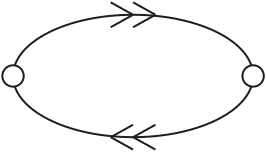
\includegraphics[scale=0.6]{1-01}
\end{figure}

The diagram has a left and right node signaling each a $U(N)$ gauge factor, so the gauge group is $SU(N)\times SU(N)$. The two arrows moving from left to right represent two different chiral fields $A_1$ and $A_2$ both in the $(\cjrep N,\rrep N)$ gauge representation, while the lower arrows are two other fields $B_1$ and $B_2$ transforming as $(\rrep N, \cjrep N)$.

Let us review briefly the structure of the action of an $\ssn \geq 1$ gauge theory; we follow \cite{wessbagger}. There is a gauge vector superfield $V$ (corresponding to an on-shell multiplet $(A_\mu,\lambda)$) with values in the algebra (that is $V = T^a V_a$ with $V_a$ in the adjoint), with an associated field-strength

\begin{equation}
	W_\alpha = - \frac{1}{4} \overline{D}_{\dot \alpha} \overline{D}^{\dot \alpha} D_\alpha V
	\label{}
\end{equation}

and the dynamics of the free vector are given by the Lagrangian

\begin{equation}
	\mathcal{L}_\mathrm{SYM} = \frac{1}{4} \int d^2 \theta \,\Tr W^\alpha W_\alpha + \operatorname{h.c.}
	\label{kineticsym}
\end{equation}

In addition, one can also include chiral superfields $\Phi_I = (\varphi_I, \psi_I)$ charged under the gauge group. These will have a kinetic term

\begin{equation}
	\mathcal{L}_\Phi = \int d^4\theta\, \Phi^\dagger_I e^{gV} \Phi_I
	\label{}
\end{equation}

which is a correction of the canonical $\int d^4 \theta \, \Phi^\dagger_I \Phi_I$ to implement gauge invariance. $g$ is the gauge coupling; note this means that one should really introduce separate gauge fields for each simple factor in the gauge group, as each one will have an independent coupling. Finally, one is free to add an interaction superpotential for the chiral fields:

\begin{equation}
	\mathcal{L}_\mathrm{int} = \int d^2 \theta\, W(\Phi) + \operatorname{h.c.}
	\label{}
\end{equation}

provided $W$ is a holomorphic, gauge invariant combination of the $\Phi_I$.

Actually, it still possible to add another term consistent with the symmetries to the Lagrangian. In the non-supersymmetric case, the Maxwell action $\frac{1}{2g_{YM}^2} \int \Tr F \wedge \hodge F$ can be supplemented by a topological term $\frac{\theta}{8\pi^2} \int \Tr F \wedge F$ fronted by a theta angle $\theta$. The same can be done in an $\ssn = 1$ gauge theory by replacing the kinetic lagrangian \eqref{kineticsym} with

\begin{equation}
	\mathcal{L}_{SYM} = \frac{1}{32\pi} \Im \left( \tau \int d^2 \theta \Tr W^\alpha W_\alpha \right)
	\label{kineticsymtau}
\end{equation}

after having introduced the complexified coupling

\begin{equation}
	\tau := \frac{\theta}{2\pi} + \frac{4\pi i}{g^2}
	\label{complexcoupling}
\end{equation}

\subsection{Renormalization and supersymmetric beta functions}

In the study of D3-brane quiver theories we will need to identify their conformal manifolds as defined in \ref{sec:scft}, or less ambitiously just its dimension. This is the number of marginal directions, deformations of the theory that preserve its superconformal invariance. In general we will have a space of parameters $(g_1, g_2, \ldots, g_\chi, \lambda_1, \ldots, \lambda_k)$ including gauge and superpotential couplings, and the conformal manifold will be the submanifolds of values of these couplings for which $\beta_{g_1} = \ldots = \beta_{g_\chi} = \beta_{\lambda_1} = \ldots = \beta_{\lambda_k} = 0$.

Thankfully, the renormalization structure of supersymmetric theories is in general vastly simplified with respect to the general case. In the case of $\ssn \geq 1$ supersymmetry, there is a remarkably simple formula for the gauge beta functions, connecting them to the anomalous dimensions of the fields:

\begin{equation}
	\beta(g_a) = - \frac{g_a^3}{16\pi^2} \frac{3 T[\mathrm{Adj}] - \sum_i T[R_i] (1- 2\gamma_i) }{1-Ng_a^2 / 8\pi^2 }\,.
	\label{NSVZ}
\end{equation}

$T[R]$ is the Dynkin index of the representation $R$ of the gauge group. The sum is over the chiral fields charged under the gauge group, and their representations and anomalous dimensions $R_i$, $\gamma_i$. This is known as the Novikov-Shifman-Vainshtein-Zakharov (NSVZ) $\beta$ function, and is known to be correct to all orders in perturbation theory \cite{Carlino:1999tc}. A further simplifying step will be possible because in addition to supersymmetry the theory has superconformal invariance, as the anomalous dimension $\gamma = \Delta - 1$ will be connected to the R-charge at conformal points according to \eqref{deltarcharge}.

For what concerns instead the $\beta$ functions for superpotential couplings, it is easy to see the scale-invariance of the action corresponds to an exact R-charge of $2$ for the superpotential. Therefore the vanishing of these $\beta$ functions is equivalent to imposing the sum of R-charges of the entering chiral fields is $2$.



We now are ready to begin our investigation of the following specific chain of theories:
\setlength\extrarowheight{12pt}
\begin{center}
\begin{tabular}{c  c  c}
	\hline
	Theory & $\ssn$ & Quiver diagram  \\\midrule \midrule
	$\ssn = 4$ Super-Yang-Mills & $4$ & \raisebox{-.4\height}{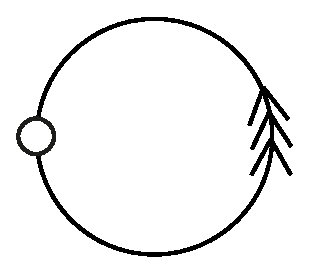
\includegraphics[scale=0.2]{4-01}}\\  
	\multicolumn{3}{c}{ $\downarrow$ $\mathbb{Z}_2$ orbifold} \\ 
	$\mathbb{C}^3/\mathbb{Z}_2$ & $2$ & \raisebox{-.4\height}{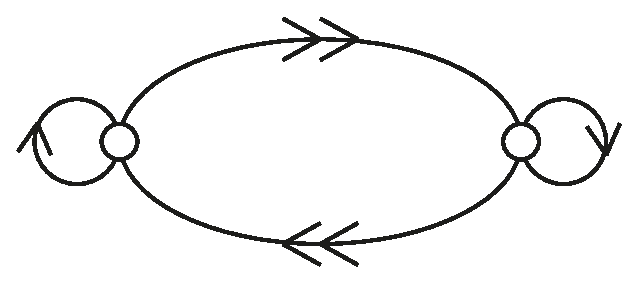
\includegraphics[scale=0.2]{2-01}} \\ 
	\multicolumn{3}{c}{ $\downarrow$ mass deformation} \\ 
	Klebanov-Witten & $1$ & \raisebox{-.4\height}{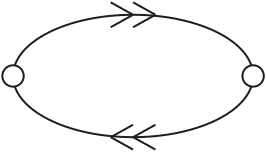
\includegraphics[scale=0.2]{1-01}}\\ 
	\multicolumn{3}{c}{ $\downarrow$ $\mathbb{Z}_2$ orbifold} \\ 
	$Y^{2,0}$ & $1$ & \raisebox{-.4\height}{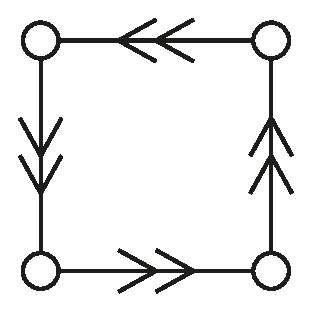
\includegraphics[scale=0.2]{3-01}}\\ 
\end{tabular}
\end{center}
\setlength\extrarowheight{0pt}
The transformations turning each theory into the next will be explained progressively.

\section{Brane stack in $\mathbb{C}^3$ and $\mathcal{N}=4$ super-Yang-Mills} \label{SYM4}

If $X_6 = \mathbb{C}^3$, the branes are invariant under half of the $16 \times 2 = 32$ IIB supercharges. This implies $\mathcal{N}=4$ for the field theory. Moreover, the theory features gluons as the massless spin-1 modes for the sector of strings stretching between brane $i$ and brane $j$ so that the gauge group is $U(N)$, as seen in \ref{sec:branestacks}. The information that the theory is a $U(N)$ gauge theory and is maximally supersymmetric is enough to uniquely fix it. Actually, since our main interest is in the IR limit, the $U(1)$ gauge factor decouples as we have explained in general, and the group is reduced to $SU(N)$.

In $\mathcal{N}=1$ language (which we employ even though the model has $\mathcal{N}=4$) the theory describes the dynamics of an $U(N)$ gauge vector supermultiplet $V_\mu$ and three complex chiral superfields $(X^a)_{i\dot j}$, $a=1,2,3$ in the adjoint of the gauge group (we will frequently omit gauge indices). These are nothing else than the parametrization of the D3-branes' position in $\mathbb{C}^3$ and therefore transform in the fundamental of $SU(3)$. The superpotential is the only one allowed by gauge and $SU(3)$ invariance,

\begin{equation} W(X) = g \epsilon_{abc} \Tr ( X^a X^b X^c) \label{sym4potential}\,;
\end{equation}

note the coupling $g$ is also the coupling of the gauge group, not an indipendent parameter. Since the theory has a single $SU(N)$ factor in the gauge group, and three fields in the adjoint (which is trivially a bifundamental with the same node at the two ends), the quiver diagram is rather simple:

\tikzset{% arrow close to the source: the 0.2 determines where the arrow is drawn
  ->-/.style={decoration={markings, mark=at position 0.5 with {\arrow{stealth}}},
              postaction={decorate}},
}

\begin{figure}[H]
	\centering
%\begin{tikzpicture}[every node/.style={circle,draw},thick,scale=1.5]
%  \node(NL) at (0,0){};
%  \draw[->-](NL.north) to [loop above, min distance=20mm, in=-45, out=45, looseness=8]	(NL.south);
%  \draw[->-](NL.north) to [loop above, min distance=24mm, in=-45, out=45, looseness=8]	(NL.south);
%  \draw[->-](NL.north) to [loop above, min distance=28mm, in=-45, out=45, looseness=8]	(NL.south);
%\end{tikzpicture}
	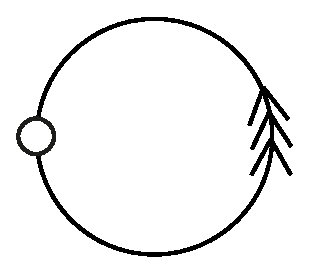
\includegraphics[scale=0.5]{4-01}
\end{figure}


Note that the obvious global symmetries, the $U(1)$ R-charge for $\ssn = 1$ and the $SU(3)$ flavour symmetry acting on the $X^a$ are actually just a subgroup of a $SU(4)$ R-symmetry group for the hidden $\ssn = 4$ supersymmetry. To make this manifest, split the $\ssn=1$ superfields as $V \rightarrow (A_\mu,\lambda)$ and $X^a \rightarrow (\phi^a,\psi^a)$, and regroup the fields as

\begin{align}
	\lambda^\alpha := (\lambda,\psi^1,\psi^2,\psi^3)\,,\quad \phi^i =: \varphi^i + i \varphi^{i+3}\,,
	\label{}
\end{align}

then $(A_\mu,\lambda^\alpha,\varphi^i)$ form an $\ssn=4$ vector supermultiplet, the components transforming respectively as $\mathbf{1}$, $\mathbf{4}$, $\mathbf{6}$ under R $SU(4)$, and in the adjoint of gauge $SU(N)$.

\subsection{Marginal deformations}

$\ssn = 4$ (maximal) supersymmetry is extremely constraining, and indeed a non-renormalization theorem (first proven nonperturbatively in \cite{seibergnr}) states the theory is exactly finite. No divergences means the $\beta$ function (one for the only gauge coupling) vanishes identically, and the theory is always superconformal. Indeed, there is a set of additional 16 supercharges beyond the standard ones. These do \emph{not} however find a direct correspondence as supersymmetries of the D3-brane system, but only of the ``near-horizon'' ($\alpha' \rightarrow 0$) geometry of the brane stack.

However, one can also discuss the vanishing of the beta function in $\ssn = 1$ language as a trivial example. We note $SU(3)$ flavour symmetry imposes that the R-charges and anomalous dimensions of the three chiral fields are equal. Then, for the superpotential to be scale invariant we need $R_W$ to be $2$, so

\begin{equation}
	R_W = 2 = R + R + R \Rightarrow R = \frac{2}{3} \Rightarrow \gamma = 0\,,
	\label{}
\end{equation}

where \eqref{deltarcharge} was used; thus, the chiral fields have canonical dimension. Then the NVSZ beta function for the gauge coupling reads

\begin{equation}
	\beta_\tau \propto 3 N - 3 N (1-2\gamma) = 3N-3N = 0\,.
\end{equation}

So, this vanishes identically, for all values of the coupling $\tau$. Thus the conformal manifold of such a theory is minimal: there is a single marginal deformation corresponding to changing $\tau$, and the theory is a SCFT for every value of this unique parameter.

\subsection{Moduli space}

One could wonder instead about the moduli space $\mathcal{M}$ of the theory. This is the space of inequivalent vacua; classically, one plugs uniform vacuum expectation values $X^a$ for the chiral fields into the action to get an effective potential:

\begin{equation}
	\mathcal{V}(X^a) = \pder{W^\dagger}{X^\dagger_a} \pder{W}{X^a} =: F^{a\dagger} F_a\,,
	\label{}
\end{equation}

which is then minimized. Since $\mathcal{V} \geq 0$ and it equals zero at the special point $X^a = 0$, its minima will coincide with its zeroes, which occurr when all of the $F^a$ vanish:

\begin{equation}
	F_a := \pder{W}{X^a}\,
	\label{fflatness}
\end{equation}

$F_a$ is known as an F-term and the conditition \eqref{fflatness} is known as an F-flatness condition.

The moduli space of \SYM is then very easy to describe. The F-term conditions simply read:

\begin{equation}
	\pder{W}{X^a} \propto \varepsilon_{abc} X^b X^c = 0\,,
	\label{}
\end{equation}

so that the space of solution is given by (VEVs of) $X^a$ that commute with eachother as $N\times N$ matrices. Therefore, they can be simultaneously diagonalized by a gauge transformation, and the $3N$ eigenvalues $x^a_I$, $I=1,\ldots,N$ are completely free. In fact, these coincide directly with the coordinates of the $N$ D3-brane on $\mathbb{C}^3$. The moduli space is $\mathbb{C}^{3N}$, or to be precise, taking into account brane indistinguishability (i.e., the residual permutation gauge symmetry after diagonalization of the $X^a$),

\begin{equation}
	\mathcal{M} = \operatorname{Sym}^N \mathbb{C}^3\,.
	\label{}
\end{equation}

In fact, this structure will always be present in D3-brane theories. Moduli space will always include a $\mmes \subset \mathcal{M}$ describing the motion of the D-branes on $X_6$, and it will be true in general that $\mmes = \operatorname{Sym}^N X_6$. However, $\mmes$ will not comprise the totality of moduli space and in more complex theories additional directions to $\mathcal{M}$ will arise.

\section{$\mathbb{C}^3/\mathbb{Z}_2$ orbifold}

We now move to a less trivial case by performing an orbifold of the background. Essentially, we act on $\mathbb{C}^3$ as such

\begin{equation}
	(z^1, z^2, z^3) \mapsto (-z^1, -z^2, z^3)
	\label{}
\end{equation}

and quotient under this $\mathbb{Z}_2$ group. This yields a Calabi-Yau manifold with a conical singularity in $z^1 = z^2 =0$. Equivalently, if the background is presented in polar coordinates as $\mathbb{R}_+ \times \mathbb{S}^5$, the orbifold produces $\mathbb{R}_+ \times (\mathbb{S}^5 / \mathbb{Z}_2)$. Our interested is then for the worldvolume theory of $N$ D3-branes placed in this singular background.

To investigate this, we consider $\tilde N = 2N$ D3-branes on $\mathbb{C}^3$, producing \SYM as seen in the previous section, then we act on the $A_\mu$ and $X^a$ fields with the $\mathbb{Z}_2$ action and select the subset of invariant fields - these will be the degrees of freedom of the orbifold theory.

We need to specify an action of $\mathbb{Z}_2$ on the gauge indices. The following choice is convenient: act on an object in the fundamental $\mathbf{\tilde N} = \mathbf{N} \oplus \mathbf{N}$ as $1$ on the first factor and $-1$ on the second. This means, for example, that having decomposed $A_\mu$ in subrepresentations its transformation under $\mathbb{Z}_2$ is

\begin{equation}
	A_\mu = \begin{pmatrix}
		A^{0,0} & A^{1,0} \\
		A^{0,1} & A^{1,1}
	\end{pmatrix} \mapsto \begin{pmatrix}
		A^{0,0} & -A^{1,0} \\
		-A^{0,1} & A^{1,1}
	\end{pmatrix}\,,
\end{equation}

where $A^{i,j}$ are $N\times N$ matrices. We see the surviving gauge fields are $A^{0,0}$ and $A^{1,1}$, adjoint for the $U(N) \times U(N)$ subgroup of $U(2\tilde N)$. The new gauge group is therefore $U(N) \times U(N)$.

The same holds for $X^3$, which becomes $\Phi := (X^3)^{0,0}$ and $\tilde \Phi := (X^3)^{1,1}$, two chiral fields each in the adjoint of one of the $U(N)$ factors.

For $X^1$, $X^2$ instead one has to take into account both the action on the gauge indices and the direct action on the $\mathbb{C}^3$ geometry. With $i=1,2$, the overall action is

\begin{equation}
	X^i = \begin{pmatrix} 
			(X^i)^{0,0} & (X^i)^{1,0} \\
			(X^i)^{1,0} & (X^i)^{1,1} 
		\end{pmatrix}\mapsto \begin{pmatrix} 
			-(X^i)^{0,0} & (X^i)^{1,0} \\
			(X^i)^{1,0} & -(X^i)^{1,1} 
		\end{pmatrix}\,,
\end{equation}

and one ends up with two pairs of chiral fields in bifundamentals, $A^i := (X^i)^{0,1}$, $B^i := (X^i)^{1,0}$, in representations $(\rrep N, \cjrep N)$ and $(\cjrep N, \rrep N)$ of $U(N)\times U(N)$ respectively. The structure of the theory can be more elegantly presented in a quiver diagram:

\begin{figure}[H]
	\centering
%\begin{tikzpicture}[every node/.style={circle,draw},thick,scale=1.5]
%  \node(NL) at (0,0){};
%  \node(NR) at (2,0){};
%  \draw[->-](NL.north) to [bend left=60]	(NR.north);
%  \draw[->-](NL.north) to [bend left=90]	(NR.north);
%  \draw[->-](NR.south) to [bend left=60]	(NL.south);
%  \draw[->-](NR.south) to [bend left=90]	(NL.south);
%  \draw[->-] (NL.south west) to [loop left, min distance=5mm, in=120, out=230, looseness=10] (NL.north west);
%  \draw[->-] (NR.south east) to [loop left, min distance=5mm, in=60, out=300, looseness=10] (NR.north east);
%\end{tikzpicture}
	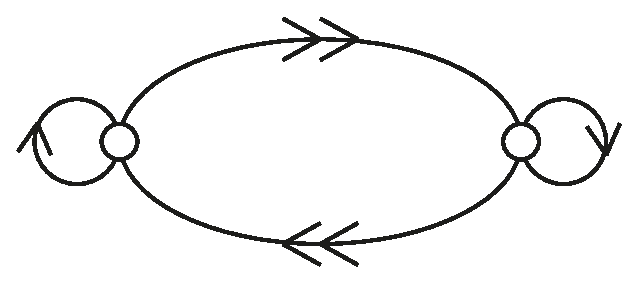
\includegraphics[scale=0.5]{2-01}
\end{figure}

The superpotential is just given by restriction of the \SYM potential \eqref{sym4potential} to the surviving fields; after some algebra

\begin{equation}
	W = \mu \left( \Tr \Phi (A_1 B_1 + A_2 B_2 ) + \Tr \tilde\Phi (B_1 A_1 + B_2 A_2) \right)
	\label{}
\end{equation}

It is clear at this point that, given the introduction of an asymmetry between $X^3$ and $X^{1,2}$, the $\ssn = 4$ R-symmetry $SU(4)$ is broken and so is maximal supersymmetry. The orbifold theory has indeed $\mathcal{N}=2$ supersymmetry \cite{Douglas}.

%
%This theory, moreover, is also superconformal at some points. The form of the potential is again fixed (there are no possible deformation consistent with the remaining symmetries) except for the overall constant $\mu$; therefore a set of parameters for the theory is given by the three couplings $(\tau_1,\tau_2,\mu)$, where we have accounted for the fact that the two gauge factors can flow independently under the renormalization group. Then, the vanishing of the $\beta_\mu$ function for the $\mu$ coupling is equivalent the R-charge of the superpotential being $2$, so that
%
%\begin{equation}
%	R_\Phi + R_A + R_B = 2\,,\quad R_{\tilde\Phi} + R_A + R_B = 2
%	\label{}
%\end{equation}
%
%which, employing $\frac{3}{2}R = 1+\gamma$ for chiral fields at a superconformal point, is equivalent to
%
%\begin{equation}
%	\gamma_\Phi + \gamma_A + \gamma_B = 0 = \gamma_{\tilde \Phi} + \gamma_A + \gamma_B\,.
%	\label{}
%\end{equation}
%
%We combine this with the vanishing of the two gauge $\beta$ functions. Using the NSVZ formula for the left node we get
%
%\begin{equation}
%	\beta \propto 3N-N(1-2\gamma_\Phi) - 2 \frac{N}{2} ( 1-2\gamma_A) - 2 \frac{N}{2} (1- 2\gamma_B) = 2 ( \gamma_\Phi + \gamma_A + \gamma_B) = 0\,,
%	\label{}
%\end{equation}
%
%and identically for the other gauge node, replacing $\Phi$ with $\tilde\Phi$. Therefore the conformal conditions are not all independent: only two independent conditions determine the conformal manifold. Since we have a three parameter space $(\tau_1, \tau_2, \mu)$, the locus of conformal points will be 1-dimensional. At a generic point $(\tau_1,\tau_2,\mu)$ in parameter space the theory will not be superconformal; however it should flow in the IR towards a point on the conformal curve.
%
%Directions along the conformal manifolds are marginal deformations of the theory, as seen before. In this case, one marginal deformation will be present.
%

We will not concentrate on the details of this $\mathbb{C}^3/\mathbb{Z}_2$ theory; we use it as a stepping stone from \SYM to the Klebanov-Witten theory, which we will introduce in the next section as a deformation of the orbifold theory.

\section{The conifold and the Klebanov-Witten model} \label{sec:KW}

In \cite{KW_SCFT} the case of $X_6$ being the conifold was studied. The conifold is a specific Calabi-Yau 3-cone defined for example as the following variety in $\mathbb{C}^4$:

\begin{equation}
	z_1^2 + z_2^2 + z_3^2 + z_4^2 = 0\,,
\end{equation}

with the K\"ahler structure inherited from the standard one on $\mathbb{C}^4$, or, after a simple change of variables:

\begin{equation}
	u v - xy = 0\,.
	\label{conifoldeq}
\end{equation}

The base can be found by quotienting by dilations $z_i \rightarrow \lambda z_i$ (with $\lambda \in \mathbb{R}_+$) and turns out to be the homogeneous space $SO(4)/U(1) = SU(2)\times SU(2) / U(1)$, where the $U(1)$ is a diagonal subgroup generated by, say, $T^3_L + T^3_R$. Topologically, this is $\mathbb{S}^2 \times \mathbb{S}^3$. We will therefore have $SU(2)\times SU(2)$ as part of the isometry group of both $Y_5$ and $X_6$, and thus will also appear as a global symmetry of the wordvolume theory. An equivalent description of the topology of the conifold is as a $U(1)$ bundle over $\mathbb{C}P^1 \times \mathbb{C}P^1 \cong \mathbb{S}^2 \times \mathbb{S}^2$; in these terms the metric on this cone is

\begin{gather}
	ds^2_6 = dr^2 + r^2 ds^2_5 \nonumber\\
	ds^2_5 = \frac{1}{9} (d\psi + \cos\theta_1 d\phi_1 + \cos\theta_2 d\phi_2)^2 + \frac{1}{6} (d\Omega_1^2 + d\Omega_2^2)\label{conifoldmetric}
\end{gather}

where $\Omega_i^2 = d\theta_i^2 + \sin\theta_i^2 d\phi_i^2$ is the metric on the $\mathbb{C}P^1_i$, and $\psi$ is the fibral coordinate with period $4\pi$.

The corresponding field theory (which we will call the Klebanov-Witten model), however, can also be found by applying a particular modification to the orbifold theory of the previous section \cite{KW_SCFT}. Let us derive the form of this SCFT in this way, and then show how the above geometry reappears from the field theory side. The modification is the addition of a relevant term to the Lagrangian, a mass for the $\Phi$, $\tilde\Phi$ adjoint fields

\begin{equation}
	\mathcal{M} = \frac{M}{2} \left( \Tr \Phi^2 - \Tr \tilde\Phi^2 \right)\,,
	\label{massterm}
\end{equation}

thus providing a possible UV completion for the $\mathbb{C}^3/\mathbb{Z}_2$ theory. These fields are then eliminated using the resulting classical equations of motion. For example,

\begin{equation}
	\pder{(\mathcal{M} + W)}{\Phi} = 0 \Rightarrow \Phi = - \frac{\mu}{M} \left( A_1 B_1 + A_2 B_2 \right)
	\label{}
\end{equation}

and analogously for $\tilde \Phi$. Finally, these are substituted back into the action, reducing the chiral fields to just $A_i$ and $B_i$ and the superpotential to

\begin{equation}
	W = \frac{\lambda}{2} \epsilon^{ij} \epsilon^{kl} \Tr \left( A_i B_k A_j B_l \right)
	\label{kwpotential}
\end{equation}

having defined $\lambda := \frac{\mu^2}{2M}$. More formally, it is argued that after the introduction of the relevant term \eqref{massterm} the $\mathbb{C}^3/\mathbb{Z}_2$ theory flows in the IR to the Klebanov-Witten model.

Therefore, the worldvolume gauge theory is a $U(N)\times U(N)$ field theory featuring two chiral doublets $A_i$, $B_j$ with $i,j = 1,2$ transforming in opposite bifundamentals, that is $A_i$ in $(N,\bar N)$ and $B_j$ in $(\bar N, N)$. The quiver diagram is simpler:

\begin{figure}[H]
	\centering
%\begin{tikzpicture}[every node/.style={circle,draw},thick,scale=1.5]
%  \node(NL) at (0,0){};
%  \node(NR) at (2,0){};
%  \draw[->-](NL.north) to [bend left=60]	(NR.north);
%  \draw[->-](NL.north) to [bend left=90]	(NR.north);
%  \draw[->-](NR.south) to [bend left=60]	(NL.south);
%  \draw[->-](NR.south) to [bend left=90]	(NL.south);
%\end{tikzpicture}
	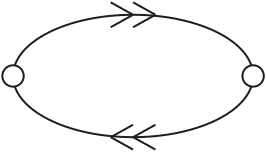
\includegraphics[scale=0.5]{1-01}
\end{figure}

The $i$ and $j$ indices, instead, are acted upon respectively by the global left and right $SU(2)$ symmetries. From the form of the superpotential and these symmetries, furthermore, it is possible to deduce the R-charges of $A_i$ and $B_i$ are $1/2$, implying a dimension of $\Delta = 3/4$ when the theory is conformal. A non-canonical scaling dimension is a symptom that the CFT will always be strongly-coupled.

It is also clear the supersymmetry has been broken further to $\ssn = 1$, since \eqref{massterm} is not $\ssn = 2$ invariant. The case at hand is thus a four-dimensional strongly-coupled field theory with minimal supersymmetry.

\subsection{Marginal deformations}\label{sec:KWmarginal}

The Klebanov-Witten theory will not be in general superconformal; it will flow through renormalization in the IR to a conformal submanifold in the space of couplings $(\lambda,\tau_1,\tau_2)$, the locus where the $\beta$ functions for these three couplings vanish. It turns out these three conditions are all equivalent. In particular, requiring either $\beta_{\tau_1} = 0$ or $\beta_{\tau_2} = 0$ and making use of the NSZV \eqref{NSVZ} this unique condition is equivalent to

\begin{equation}
	3 T[\mathrm{Adj}] - \sum_i T[R_i] ( 1- 2\gamma_i) = 0\,.
	\label{}
\end{equation}

When evaluating this, care should be taken with the fact that $A_i$ and $B_j$ have a $U(N)_2$ index which is uncharged under $U(N)_1$ and must be summed over. Noting $\gamma_{A_1} = \gamma_{A_2}$ and $\gamma_{B_1} = \gamma_{B_2}$ because of the global flavour $SU(2)\times SU(2)$ symmetry, this gives

\begin{equation}
	\gamma_A + \gamma_B + \frac{1}{2} = 0\,.
	\label{}
\end{equation}

Being $\gamma_{A,B}$ functions of the couplings, this equation defines a critical 2-surface in parameter space. Switching to R-charges, this means

\begin{equation}
	R_A + R_B = 1\,,
	\label{}
\end{equation}

but this is also the equation for the vanishing of the $\beta$ function for the superpotential coupling $\lambda$, since $R_W = 2$ is just

\begin{equation}
	R_A + R_B + R_A + R_B = 2\,.
	\label{}
\end{equation}

Thus, since the three conditions are equivalent, the final conformal manifold is the locus of a single equation in three variables $(\lambda,\tau_1,\tau_2)$ and is then two-dimensional. Therefore there will be two marginal deformations of the theory.

\subsection{Global $U(1)$} \label{sec:kwuone}

Let us comment briefly on the whereabouts of the abelian gauge factors of $U(N) \times U(N)$ under RG flow towards the infrared. Denoting as $T^1$ and $T^2$ the generators of the two trace $U(1)$ of the left and right nodes, it is clear $T^1+T^2$ is the overall completely decoupled $U(1)_\text{trace}$ that we can safely ignore. The only remaining abelian factor is generated by $B = T^1 - T^2$. This symmetry is non-anomalous; since it is an abelian gauge interaction with massless charged matter, under RG flow towards the infrared its coupling vanishes and thus freezes into a rigid $U(1)_\text{baryonic}$ in the IR. We call this charge, corresponding to the symmetry

\begin{equation}
	A_i \rightarrow e^{i\theta} A_i\,,\quad B_i \rightarrow e^{-i\theta} B_i
	\label{}
\end{equation}

a baryon number. This quantum number will become important in classifying gauge invariant operators, as we will see shortly.

\subsection{Moduli space}

Position in moduli space $\mathcal{M}$ should be parametrized by the expectation values of gauge-invariant operator (hadrons). This should be obtained, as it was sketched for \SYM, by considering the locus of minima of the effective potential $\mathcal{V}$ in the space of VEVs of the chiral fields, and then quotienting by complexified gauge transformations. Taking for the moment a general $\ssn=1$ theory with gauge generators $T^a$ and chiral fields $\phi^i$, the effective potential can be found to be

\begin{equation}
	\mathcal{V}(\phi) \;=\; \frac{g_a^2}{2} (\phi^\dagger T^a \phi)^2 + \pder{W^\dagger}{\phi^\dagger_i} \pder{W}{\phi^i} \; =:\; \frac{g_a^2}{2} (D^a)^2 + F^\dagger_i F^i
	\label{effpotential}
\end{equation}

We have defined the F-terms and the D-terms:

\begin{align}
	F^i &= \pder{W}{\phi^i}\,,\label{ftermdef}\\
	D^a &= \sum_i \phi_i^\dagger T^a \phi_i\,.\label{dtermdef}
\end{align}

Again, $\mathcal{V}$ will be minimum when $\mathcal{V}=0$, thus when the F-term and D-term vanish, conditions we will call F-flatness and D-flatness. The space of simultaneous solutions to $F^i = D^a = 0$, quotiented by gauge transformations, will be moduli space $\mathcal{M}$.

Specializing to the Klebanov-Witten model, $D^a = 0$ will hold only with $a$ spanning over generators of $SU(N) \times SU(N)$, not involving the abelian factors $U(1)_1\times U(1)_2 = U(1)_\text{trace} \times U(1)_\text{baryon}$, since according to our discussion in section \ref{sec:kwuone} these do not survive as gauge symmetries in the IR. The D-term of $U(1)_\text{trace}$ has no significance, since this is completely decoupled and vanishes identically. The baryon D-term instead gets relaxed

\begin{equation}
	D^{U(1)_\text{baryon}} = \xi
	\label{}
\end{equation}

where $\xi$ is an arbitrary parameter. Actually, $\xi$ is a modulus, parametrizing a direction in $\mathcal{M}$ itself. Indeed, it is the only additional direction in $\mathcal{M}$ to those along $\mmes$, which is a strict subset of the KW moduli space. Let us determine $\mathcal{M}$, identify $\mmes$ and verify these claims. The vanishing of the F-terms \eqref{ftermdef} and D-terms \eqref{dtermdef}, specialized to the particular case, are

\begin{equation}
	\epsilon^{ij} A_i B_a A_j = \epsilon^{ij} B_i A_a B_j = 0
	\label{}
\end{equation}

\begin{equation}
	A_i A_i^\dagger - B_i B_i^\dagger = A^\dagger_i A_i - B^\dagger_i B_i = \xi \mathbbm{1}
	\label{}
\end{equation}

the equation have to be understood to hold for VEVs. Note the first and second D-term condition are respectively from the left and right gauge group. 

Consider the subset of $\mathcal{M}$ with $\xi = 0$; our claim is this is precisely $\mmes$. To reinterpret the F-flatness condition, we introduce the four matrices $\Phi_{ij} = A_i B_j$ and note

\begin{align}
	\left[ \Phi_{ij} , \Phi_{jk} \right] = 0\\
	\Phi_{11} \Phi_{22} = \Phi_{21}\Phi_{12}
	\label{}
\end{align}

which can be immediately checked to follow from the vanishing of the F-term. Since these commute, they can be simultaneously diagonalized and their $N$ eigenvalues (one for each brane) satisfy the conifold's equation \eqref{conifoldeq}:

\begin{equation}
	\phi^I_{11} \phi^I_{22} = \phi_{21}^I \phi_{12}^I
	\label{}
\end{equation}

so these quite literally parametrize the motion of the $N$ D3-branes on the background cone. These actually determine the VEVs of mesonic operators, mesons\footnote{The meson/baryon terminology is meant to be a direct generalization of the concept of QCD hadrons. A QCD meson is to a first approximation built from two quarks as a symmetric product $\ket{M} \sim \delta^i_{\,j} \ket{q^i \overline q_j} + \mathcal O (gluons)$, while a baryon is $\ket{B} \sim \epsilon_{ijk} \ket{q^i q^j q^k}$. In general, $SU(N)$-singlets can be built by contracting gauge indices either with the symmetrical $\delta^i_j$ or the antisymmetric $\epsilon_{a_1 \ldots a_N}$.} being generated by prototipical trace operators:

\begin{equation}
	M_{(ab\ldots),(ij\ldots)} =	\Tr\left( (A_a B_i)(A_b B_j)\cdots \right)\,.
	\label{}
\end{equation}

This justifies the terminology of ``mesonic moduli space'' for the submanifold $\mmes$ of $\mathcal{M}$ they describe.

Note mesons are built by tracing over closed loops in the quiver diagram to make a gauge-invariant operator. All of these operators are actually expressable as products of $\Phi$ matrices, and as it was shown, only $3$ out of $4$ of those are independent. In the end, there are (accounting for gauge indices) $3N$ independent mesons whose VEVs parametrize mesonic moduli space, coincident with the $\operatorname{Sym}^N C$, where $C$ is the conifold.

Operators of non-zero baryon number can also be constructed by using the antisymmetric invariant gauge tensor $\epsilon^{a_1\ldots a_N}$, as such:

\begin{equation}
	\mathcal{B}^A_{[k]} = \epsilon^{a_1\ldots a_N} \epsilon_{b_1\ldots b_n} (A_1)_{a_1}^{b_1} \ldots (A_1)^{a_k}_{b_k} (A_2)^{a_{k+1}}_{b_{k+1}} \ldots (A_2)^{b_N}_{a_N}
	\label{}
\end{equation}

where we have displayed gauge indices on the $A$ fields. There are only $N+1$ different assignment for the $SU(2)$ indices because of antisymmetry, so that there are $N+1$ fundamental baryons of the form of $\mathcal{B}^A$. The same could be done by swapping the two gauge groups and using $B$ fields, to get additional $N+1$ $\mathcal{B}^B$ baryons. These all have baryon number $N$ under $U(1)_\text{baryonic}$ while mesons have baryon number $0$.

All gauge-invariant operators in the theory are built out of these fundamental mesons, fundamental baryons, and their respective antiparticles (made out of the conjugate fields $A^\dagger$, $B^\dagger$. However, as we have anticipated, we only expect $g-1 = 1$ baryonic VEV to be independent. This VEV will be associated with the resolution of the cone singularity into a $\mathbb{CP}^1 \cong \mathbb{S}^2$, and will essentially coincide with $\xi$. To see an example of this deformation of the background geometry, let us set $\xi$ to a constant nonzero value. Then hypothesizing for simplicity that the $A_1, A_2, B_1, B_2$ matrices commute, applying F-term conditions we get that each set of eigenvalues satisfies

\begin{equation}
	a_1/a_2 = b_1/b_2
	\label{}
\end{equation}

So that $a_i$ and $b_i$ are proportional vectors of $\mathbb{C}^2$, therefore

\begin{equation}
	a_i = a e^{i\theta_A} n_i, \quad \quad b e^{i\theta_B} n_i
	\label{}
\end{equation}

where $a,b$ are real and $n_i$ belongs to a $\mathbb{CP}^1$. The phases are cancelled by modding gauge invariance, and $a$ and $b$ then are involved in the D-term:

\begin{equation}
	a^2 - b^2 = \xi
	\label{}
\end{equation}

so that essentially our mesonic VEVs are composed of $N$ copies of one non-compact radial coordinate (say, $a$) and a point on $\mathbb{CP}^1$. This means the conical singularity has disappeared to be replaced by a two-cycle on which the branes can move.

A more thorough investigation of the geometry probed by these mesonic directions when $\xi$ has a non-zero value would show the D3-branes are moving on the geometry of the resolved conifold, the metric \cite{PandoZayas}

\begin{equation}
	ds_6^2 = \kappa^{-1} dr^2 + \frac{1}{9} \kappa r^2 (d\psi + \cos\theta_1 d\phi_1 + \cos\theta_2 d\phi_2)^2 + \frac{1}{6} r^2 d\Omega_1^2 + \frac{1}{6} (r^2 + a^2 ) d\Omega_2^2\label{resolvedconifold}
\end{equation}
\begin{equation}
	\kappa(r) = \frac{r^2 + 9a^2}{r^2 + 6a^2}
	\label{}
\end{equation}

parametrized by a modulus $a$. Turning on the $\xi$ modulus corresponds to increasing $a$ (in fact, the two are proproportional \cite{MZ}), and to the blow up of the two-sphere at $r=0$. Instead, for $a=0$ one recovers the singular conifold \eqref{conifoldmetric}.

Thus, we have uncovered the following structure for $\mathcal{M}$. It is a $(3N + 1)$-dimensional\footnote{There is an obvious dimensional mismatch in that the complex modulus $\xi$ corresponds to a real parameter $a$ in the metric. It turns out that when the real part of a modulus maps to a K\"ahler deformation, the imaginary part describes instead a modulus for the $C_4$ Ramond-Ramond form; we will explain more in chapter \ref{chap:heft}} complex manifold on which one can define the coordinate $\xi$, a baryonic modulus. The $3N$-submanifold at $\xi = 0$ is $\mmes$, which is equal to the symmetric product of $N$ copies of the conifold and is parametrized by $3N$ complex moduli, VEVs of particular combinations of mesonic operators, that can be identified with the positions of the threebranes. If instead one consider a constant but nonzero value $\xi = \xi^*$ for the baryonic modulus, the same mesonic directions define a submanifold with the structure of the symmetric product of $N$ copies of the \emph{resolved} conifold \eqref{resolvedconifold}.

The explicit form of the baryon generating this deformation in terms of the fundamental hadrons is very challenging to determine \cite{Forcella}; fortunately, we will not need it for our purposes. In any case, all of this information will be clarified in the context of holography.



\section{The $Y^{2,0}$ orbifold theory}\label{sec:squares}

The same construction on a $\mathbb{Z}_2$ orbifold of the conifold yields a quiver gauge theory which will be the main interest of this work. This theory has a few interesting additional features with respect to the Klebanov-Witten model while remaining relatively simple, thus being an optimal candidate for the investigation of its effective low-energy theory, which we will perform in chapter \ref{chap:y20}. It is, like the conifold theory, an $\ssn = 1$ SCFT but boasts three baryonic moduli, of which one has no clear geometric interpretation, and two anomalous $U(1)$s. We now describe this theory and extract these features.

The geometry of the base of the cone is very simply introduced in polar coordinates as 

\begin{gather}
	ds^2_6 = dr^2 + r^2 ds_5^2\nonumber\\
	ds^2_5 = \frac{1}{9} (d\psi + \cos\theta_1 d\phi_1 + \cos\theta_2 d\phi_2)^2 + \frac{1}{6} (d\Omega_1^2 + d\Omega_2^2)\label{y20conemetric}
\end{gather}

i.e., exactly the same metric in form as the conifold, but with $\psi$ now with period $2\pi$. This background and the resulting worldvolume field theory are just one entry $Y^{2,0}$ of an infinite class $Y^{p,q}$ of examples introduced in \cite{benvenutiInfinite}. (To be precise, we will use $Y^{2,0}$ to refer to the 5-dimensional base \eqref{y20conemetric}, following \cite{ytoozero}, and $X^{2,0}$ for the corresponding cone).

Following an identical procedure to that performed for the $\mathbb{Z}_2$ orbifold of \SYM, we can deduce the quiver diagram splits to yield four doublets $A_i$, $B_i$, $C_i$, $D_i$ of bifundamental chiral fields stretching in a square between four nodes:

\begin{figure}[H]
	\centering
%\begin{tikzpicture}[every node/.style={circle,draw},thick,scale=1.5]
%  \node(NL) at (0,0){};
%  \node(NR) at (2,0){};
%  \node(NDR) at (2,2){};
%  \node(NDL) at (0,2){};
%  \draw[->-](NL.east) to [bend right=20]	(NR.west);
%  \draw[->-](NL.east) to [bend left=20]	(NR.west);
%  \draw[->-](NR.north) to [bend right=20]	(NDR.south);
%  \draw[->-](NR.north) to [bend left=20]	(NDR.south);
%  \draw[->-](NDR.west) to [bend right=20]	(NDL.east);
%  \draw[->-](NDR.west) to [bend left=20]	(NDL.east);
%  \draw[->-](NDL.south) to [bend right=20]	(NL.north);
%  \draw[->-](NDL.south) to [bend left=20]	(NL.north);
%\end{tikzpicture}
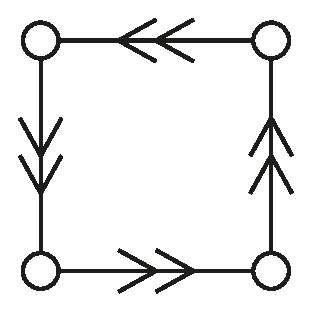
\includegraphics[scale=0.5]{3-01}
\end{figure}

so that the gauge group is $SU(N)^4$. The superpotential can be again obtained by truncation, yielding

\begin{equation}
	W = \lambda \epsilon^{ij} \epsilon^{kl} \Tr\left( A_i B_k C_j D_l \right)
	\label{squaresuperpotential}
\end{equation}

from which it is clear that the $SU(2) \times SU(2)$ isometry of the cone, corresponding to a global flavour symmetry of the field theory, must now act as

\begin{align}
	\begin{split}
		A_i \in (\rrep 2, \rrep 1)\\
		B_i \in (\rrep 1, \rrep 2)\\
		C_i \in (\rrep 2, \rrep 1)\\
		D_i \in (\rrep 1, \rrep 2)
	\end{split}
	\label{flavoursquare}
\end{align}

Note \eqref{squaresuperpotential} is also the only possible superpotential allowed by this symmetry \cite{Benvenutifourcycles}, so that the theory can also be constructed by starting with the flavour symmetry as an assumption.

\subsection{Global $U(1)$s} \label{sec:squaresuones}

The novelty in this model is the appearance of anomalous $U(1)$s. In detail, the ultraviolet theory has the original gauge group $U(N)^4 \cong U(1)_1 \times U(1)_2 \times U(1)_3 \times U(1)_4 \times SU(N)^4$. Of the four abelian $U(1)$s, the overall trace factor\footnote{With the notation $U(1)_a + U(1)_b$ we mean the $U(1)$ generated by the sum of the generators $T_a$ and $T_b$ of $U(1)_a$ and $U(1)_b$ respectively.}

\begin{equation}	
	U(1)_\text{trace} := U(1)_1 + U(1)_2 + U(1)_3 + U(1)_4
	\label{}
\end{equation}

has no charged fields and is completely decoupled from the theory. The other three independent combinations have a potential to develop an anomaly arising from $U(1)_a-SU(N)_b^2$ triangle diagrams; each chiral field in representation $R$ provides a contribution to the anomaly proportional to the group-theoretical factor \cite{terningmodernsusy}

\begin{equation}
	A_R^{ab;ij} := \Tr \left( Q_R^a \left\{T_R^i, T_R^j\right\} \right)
	\label{}
\end{equation}

where $Q_R^a$ is the generator of the $U(1)_a$ of interest, and $T_R^i$, $T_R^j$ are generators of $SU(N)_b$ in representation $R$. For any given gauge node $SU(N)_b$, it is then clear that the total anomaly is then proportional to the difference between the charges of the incoming and outgoing chiral fields under the $U(1)_a$

\begin{equation}
	A_\text{total}^{ab} \propto Q^a_\text{in} - Q^a_\text{out}
	\label{}
\end{equation}

so that we can immediately identify one non anomalous $U(1)$:

\begin{equation}
	U(1)_B := U(1)_1 + U(1)_3 \cong U(1)_2 + U(1)_4\,.
	\label{}
\end{equation}

The last congruence is up to shifts by $U(1)_\text{trace}$. $U(1)_B$ is thus a sensible abelian gauge factor, in fact the same already present in the Klebanov-Witten theory, and flows in the infrared into a rigid symmetry, which we define as a baryon number. The baryonic charges of $(A_i,B_i,C_i,D_i)$ are respectively $(+1,-1,+1,-1)$.

The other two independent $U(1)$s are anomalous. They are not uniquely identified since they can be shifted by $U(1)_\text{trace}$ and $U(1)_B$ or mixed with each other; one presentation would be

\begin{equation}
	U(1)_\text{AN,1} := U(1)_1 - U(1)_3\,,\quad U(1)_\text{AN,2} := U(1)_4 - U(1)_2\,.
	\label{}
\end{equation}

Thus, the charge assignments are as follows

\begin{center}
	\begin{tabular}[]{c|c}
		charges of $A$, $B$, $C$, $D$ & $U(1)$ \\ \hline \hline
		$(\;\,\;0\,,\;\,\;0\,,\;\,\;0\,,\,\;\;0\,)$ & $U(1)_\text{trace}$ \\  \hline
		$(+1,-1,+1,-1)$ & $U(1)_B$ \\ 
		$(+1,+1,-1,-1)$ & $U(1)_\text{AN,1}$ \\
		$(+1,-1,-1,+1)$ & $U(1)_\text{AN,2}$
	\end{tabular}
\end{center}

We have already commented on how the non-anomalous abelian factor becomes a rigid global symmetry flowing down to the IR. However, the anomaly of the other two abelian gauge symmetries is worrying as it would make the theory inconsistent. Actually, it turns out these anomalies are cancelled at the level of the supergravity background by the contribution of axionic fields charged under the anomalous $U(1)$s; in particular the $X^{2,0}$ cone has a 2-cycle $S$ and a 4-cycle $E$ such that the integrals

\begin{equation}
	\phi_1 = \int_S A_2 \quad \phi_2 = \int_E A_4
	\label{}
\end{equation}

of some supergravity 2- and 4-form $A_2$, $A_4$ constitute dynamical four-dimensional fields $\phi_1(x^\mu)$, $\phi_2(x^\mu)$ which cancel the anomaly, in a form of the Green-Schwarz mechanism\footnote{This is actually expected, as string theory is quantum consistent and no configuration in it can display anomalies.}. However, these fields transform as axions under the two anomalous $U(1)$, and so break the corresponding symmetry in a St\"uckelberg mechanism, thus the corresponding photons become massive.

Therefore these do not exist anymore as gauge symmetries in the IR. They persist in the IR theory as rigid symmetries of the classical Lagrangian, though broken by quantum effects. Since they are not gauged, the anomaly does not make the theory inconsistent, and does indeed occurr. Thus, even though the \emph{gauge} anomaly of these abelian factor is canceled in the string theory by the axion, the resulting global $U(1)_\text{AN}$ symmetries are still anomalous.

\subsection{Marginal deformations} \label{sec:squaresmarginal}

We turn to the study of marginal deformations. Again, the flavour symmetry \eqref{flavoursquare} guarantees $\gamma_{A_1} = \gamma_{A_2} = \gamma_A$ and so on. This time three of the four gauge $\beta$ functions are independent:

\begin{align}
	\begin{split}
\beta_1 = 0 \quad	& \Rightarrow  \quad	\gamma_A + \gamma_D + \frac{1}{2} = 0\,, \\
\beta_2 = 0 \quad	&  \Rightarrow	\quad	\gamma_B + \gamma_A + \frac{1}{2} = 0\,, \\
\beta_3 = 0 \quad	&  \Rightarrow	\quad	\gamma_C + \gamma_B + \frac{1}{2} = 0\,.
	\end{split}
\end{align}

In addition, $\beta_\lambda = 0$ is also not independent: at any superconformal point, $\frac{3}{2}R - 1 = \gamma$, so that the condition that $W$ be scale invariant, which is equivalent to it having R-charge $2$, becomes

\begin{equation}
	\begin{split}
	2 = R_W = R_A + R_B + R_C + R_D \\\Rightarrow \gamma_A + \gamma_B + \gamma_C + \gamma_D + 1 = 0
	\label{}
\end{split}
\end{equation}

which is indeed equivalent to the above system. Three independent equations in the five-parameter space of $(\tau_1,\tau_2,\tau_3,\tau_4,\lambda)$ define, again, a critical 2-submanifold.

\subsection{Moduli space}\label{sec:squaresmoduli}

Turning to the investigation of the moduli space, the F-term condition for the given superpotential read

\begin{align}
	\begin{split}
	A_\alpha B_\sigma C_\beta \epsilon^{\alpha\beta} = 0 \\
	B_\alpha C_\sigma D_\beta \epsilon^{\alpha\beta} = 0 \\
	C_\alpha D_\sigma A_\beta \epsilon^{\alpha\beta} = 0 \\
	D_\alpha A_\sigma B_\beta \epsilon^{\alpha\beta} = 0 
	\label{Ftermssquare}
\end{split}
\end{align}

For what concerns the D-terms, as in the case of the conifold we only need to consider those relative to the true gauge symmetries of the IR theory, so those for $SU(N)^4$. As we have seen in the previous section, the $U(1)$ factors either become rigid or broken. Accordingly, the abelian D-terms get relaxed into four arbitrary parameters:

\begin{equation}
	D^{U(1)_i} = \xi^i\,,\quad i = 1,2,3,4
	\label{}
\end{equation}

Combining this information, the vanishing of the D-term takes the form

\begin{align}
	\begin{split}
		A_i A^\dagger_i - B_i B^\dagger_i = \xi_1 \mathbbm{1} \\
		B_i B^\dagger_i - C_i C^\dagger_i = \xi_2 \mathbbm{1} \\
		C_i C^\dagger_i - D_i D^\dagger_i = \xi_3 \mathbbm{1} \\
		D_i D^\dagger_i - A_i A^\dagger_i = \xi_4 \mathbbm{1}
	\end{split}
	\label{Dtermssquare}
\end{align}

with the constraint $\sum_i \xi_i = 0$ (obvious by summing the four equations \eqref{Dtermssquare}, and clear since it corresponds to the trace $U(1)$). Thus $\xi^i$ include $3$ independent baryonic moduli.

We already expect that the solutions to \eqref{Ftermssquare} and \eqref{Dtermssquare} (modulo gauge symmetry) should be parametrized by $3N$ mesonic operators measuring the positions of the branes and $3$ baryonic operators associated with the $\xi^i$, and that for $\xi^i = 0$ we recover $\mmes$ corresponding to the motion of the branes on the singular $X^{2,0}$ \eqref{y20conemetric}. Instead, for any generic non-zero constant values of $\xi^i$, the $3N$ mesons should describe the motion of $N$ D-branes on the general resolution of the cone. 

Let us investigate the geometry of the latter by taking $\xi^i$ to have generic non-zero values (with $\sum_i \xi = 0$). Again we make the simplifying assumption the eight $A, B, C, D$ matrices commute and can be simultaneously diagonalized. So, for each of the $N$ rows of corresponding eigenvalues F-flatness \eqref{Ftermssquare} reads:

\begin{align}
	a_1/a_2 = c_1/c_2 && b_1/b_2 = d_1 / d_2
	\label{}
\end{align}

thus again $a_\alpha \propto c_\alpha$ and $b_\alpha \propto d_\alpha$, so we can ``projectivize'':

\begin{align}\begin{split}
		a_\alpha = a \, e^{i\theta_A} n_\alpha \quad b_\alpha = b \, e^{i\theta_B} n_\alpha \\
		c_\alpha = c \, e^{i\theta_C} m_\alpha \quad d_\alpha = d \, e^{i\theta_D} m_\alpha 
	\end{split}\end{align}

and again the phases are modded out by gauge symmetry, and the $a, b, c, d$ real numbers are reduced to a single coordinate (schematically $r^2$) by the three independent D-flatness conditions. Therefore the resolved geometry of the singularity is now $\ess^2 \times \ess^2$, parametrized by the $(n^I_\alpha,m^I_\alpha)$ ($I=1,\ldots,N$) coordinates of the $N$ D3-branes. Thus again for generic values of the $\xi_i$ the structure of mesonic moduli space encodes the information that the branes are moving on a resolved version of $X^{2,0}$, where the singularity has been smoothed out into an $\ess^2 \times \ess^2$.

More specifically, there are actually two moduli describing deformations of the background cone \cite{Benvenutifourcycles}. One considers the general Calabi-Yau deformation of $Y^{2,0}$, which is given by \cite{PandoZayasy20}

\begin{equation}
	\begin{split}
	ds^2 = \kappa^{-1}(r) dr^2 + \frac{1}{9} \kappa(r) r^2 \left( d\psi + \cos\theta_1 d\varphi_1 + \cos\theta_2 d\varphi_2 \right)^2 \\
	+ \frac{1}{6} r^2 d\Omega_1^2 + \frac{1}{6}(r^2 + a^2) d\Omega_2^2\,,
	\label{genCYy20cones}
\end{split}
\end{equation}

\begin{equation}
	\kappa(r) = \frac{1 + \frac{9a^2}{r^2} - \frac{b^6}{r^6}}{1 + \frac{6a^2}{r^2}}\,.
	\label{}
\end{equation}

It can be seen that the singular $Y^{2,0}$ cone is obtained as the two moduli $a$, $b$ vanish. Turning on the $b$ modulus the volume of the four-dimensional base $\ess^2\times \ess^2$ is increased (one speaks of a blow up) and the singular tip\footnote{This does not actually lie at $r=0$ because of the way the $r$ coordinate is defined, rather it corresponds to $\kappa(r) = 0$; we will clarify this in our study of the $Y^{2,0}$ resolved geometry in chapter \ref{chap:y20}} of the cone is resolved as an $\ess^2 \times \ess^2$. The modulus $a$ instead controls the relative volume of the two spheres. Therefore there are also specific values of $(a,b)$ (or, equivalently, of the $\xi_i$) such that we have a ``partial'' resolution where only one of the spheres is blown up and branes move on an $\ess^2$; this is the modulus inherited from the conifold.

In this case, the presence of $g-1 = 3$ independent $\xi$ parameters (matching with three independent baryons) should perplex, as we have just seen the resolutions are parametrized by \emph{two} moduli. In fact, the general Calabi-Yau deformation of the $Y^{2,0}$ metric will indeed depend on two moduli. In this case, the third modulus is not interpretable as due to deformation of the background metric, but is actually connected to the moduli of IIB two-form fields. We will review this fact in a holographic context.

For completeness we adapt the construction of hadronic operators. We note fundamental mesons are now built using $ABCD$ loops (omitting $SU(2)^2$ indices):

\begin{equation}
	M = \Tr \left( (ABCD)(ABCD) \ldots \right)
	\label{}
\end{equation}

and four classes of fundamental baryons can be introduced as before

\begin{equation}
	\mathcal{B}_{[k]}^A = \epsilon^{a_1\ldots a_N}\epsilon_{b_1 \ldots b_N} (A_1)^{b_1}_{a_1} \ldots (A_2)^{b_N}_{a_N}
	\label{}
\end{equation}

where the first $k$ instances of $A$ have $SU(2)$ index $1$ and the remaining $N - k$ have $2$. Again $k = 0, \ldots, N$ means $N+1$ different $\B^A$ baryons. This can be repeated for $\mathcal{B}^B$, $\mathcal{B}^C$, $\mathcal{B}^D$. Thus, we find $4$ classes of $N+1$ fundamental baryons each. Similarly to the previous case, we expect the VEV of only three of these baryons to be truly indepedent and a suitable triplet of combinations should generate the three aforementioned flat shifts. We will verify this in a holographic context in chapter \ref{chap:y20} when we will map these VEVs to effective fields.

\section{Towards the general case}\label{sec:conesgeneral}

The properties introduced with the previous examples of field theories can be reexamined for the general case of a theory arising from D3-branes on $\mathbb{R}^{1,3} \times X_6$.

For example, we can provide a more systematic description of moduli space, so the space of distinct vacua. Because of supersymmetry, the quantum moduli space will often coincide with the classical one, which is intuitively the space of minima of the potential quotiented by gauge transformations. As (see \eqref{effpotential})

\begin{equation}
	\mathcal{V} = \frac{g_a^2}{2} (D^a)^2 + F^\dagger_i F^i
	\label{}
\end{equation}

the minima occur when the VEVs of the chiral fields $\phi_i$ satisfy both the F-flatness conditions

\begin{equation}
	F^i = \pder{ W}{\phi_i} = 0
	\label{}
\end{equation}

and the D-flatness conditions

\begin{equation}
	D^a = - \sum_i \phi_i^\dagger T^a \phi_i = 0
\end{equation}

where $T^a$ are the gauge generators. The space $\mathcal{M}$ of solutions of both F and D-flatness conditions (modulo gauge transformations) will be a complex manifold, the moduli space.

A subspace of $\mathcal{M}$ is given by the so-called mesonic moduli space $\mmes$. Points of $\mmes$ will correspond to the position of the $N$ branes on the background cone - therefore $\dim_\mathbb{C} \mmes = 3N$. In fact, $\mmes = \operatorname{Sym}^N X_6$, where the symmetric product has to be taken because of brane indistinguishability.

As it was seen in the explicit examples, however, in general the moduli space is not exhausted in the purely mesonic directions; the additional ``baryonic'' directions appear from the relaxation of the D-terms corresponding to the abelian factors $U(1)^\chi$, because these do not appear as gauged symmetries in the IR theory.

Curiously, the reason for this can be different for each $U(1)$. The situation is as follows:

\begin{itemize}
	\item Part of the $U(1)$ factors are non-anomalous, and under RG flow their coupling vanishes and become rigid global baryonic symmetries.
	\item The rest of the $U(1)$ are actually anomalous, with the anomaly arising from $U(1)$-$SU(N)_i$-$SU(N)_j$ triangle diagrams. The anomaly is actually cancelled by a supergravity axionic field as explained in section \ref{sec:kwuone}, and the associated photon is made massive by a St\"uckelberg mechanism \cite{Martelli:sbv}.
\end{itemize}

In a holographic context we will be able to provide an explanation of the cancellation of this anomaly and also relate the number of anomalous and non-anomalous $U(1)$s to the topology of the cone; for now we are satisfied with knowing their D-flatness condition is relaxed and one is left with only the D-term for the $SU(N)^\chi$ part. So

\begin{align}
	D^a_{SU(N)^\chi} = 0 && D^{U(1)_i} = V^i
	\label{}
\end{align}

($i=1,\cdots,\chi$). $V^i$ are classically functions of the fields and in the quantum version will be gauge-invariant operators. Their $g$ VEVs $\langle V^i \rangle =: \xi^i$ will parametrize the missing flat directions of moduli space. To be precise, however, since the overall trace $U(1)$ (generated by the sum of the generators of the $g$ abelian trace factors) is completely decoupled, and the relative D-term $D^{U(1)_1} + \ldots D^{U(1)_\chi}$ vanishes identically, we have to impose $\sum \xi^i = 0$. Therefore that there are really only $\chi-1$ baryonic moduli, and only $\chi(N^2-1)+1$ independent remaining D-flatness conditions.

Thus we conclude $\dim \mathcal M = 3N + g - 1$. While the $3N$ mesonic directions have a direct geometrical interpretation as D3-brane movement, the baryonic directions correspond in terms of the superstring description to deformations of the $X_6$ background metric itself - generally resulting in a resolution of the conical singularity.

A different kind of feature is the presence of marginal deformations of the theory. As explained, the quantization of classically conformal field theories produces quantum systems that are only conformal in a conformal submanifold of the space of parameters. Therefore there will be a set of deformations of the couplings of the field theory (gauge and superpotential) that keeps the theory conformal, and the number will equate the dimension of the conformal manifold. These marginal deformations thus parametrize motion along the conformal variety. 

We have already seen in practice how the counting of marginal directions is very easy for this type of superconformal quiver theories thanks to the NSVZ $\beta$ function \eqref{NSVZ} and the dimension/R-charge relationship \eqref{deltarcharge} for chiral operators. However, it turns out to be non-trivial to guess how many of these conditions are actually independent in the general case. Thus, no ``fits-all'' procedure for counting marginal deformations is known; we just limit ourselves to stating the conjectural relationship with the topology of the cone:

\begin{equation}
	\text{\# of marginal deformations} = b_3(Y_5) + 1\,,
	\label{nummarginal}
\end{equation}

which has a clearer interpretation in holography, but no general proof purely from the field theory side. We note \eqref{nummarginal} holds for our list of examples: $b_3(\ess^5) = 0$ and \SYM has $1$ marginal deformations, $b_3(\ess^2 \times \ess^3) = {b_3(\ess^2 \times \ess^3 / \mathbb{Z}_2)} = 1$ and indeed both the KW and the $Y^{2,0}$ models have $2$ marginal directions.

Finally, we recap all information acquired for our chain of example theories:

\begin{center}
	\begin{tabular}[]{cccccc}
Theory & $Y_5$	& gauge group &non-an. $U(1)$s & an. $U(1)$s & $\dim \mathcal{M}$ \\	\midrule \midrule
\SYM	& 	$\ess^5$   & $SU(N)$	& $0$	 & $0$  & $3N$ \\
KW	& 	$\ess^2\times\ess^3$   & $SU(N)^2$	& $1$	 & $0$  & $3N+1$ \\
$Y^{2,0}$	& 	$\ess^2\times\ess^3/\mathbb{Z}_2$   & $SU(N)^4$	& $1$	 & $2$  & $3N+3$ \\
	\end{tabular}
\end{center}
